\chapter{Introduction}
\label{Introduction}

Phages are small viruses on the order of 27-190nm that infect and lyse (kill) specific bacteria. 
Phages act as nature's anti-microbial defense, but also impact bacteria evolution and resource turnover. 
There are various medical and industrial applications for phages to control bacterial growth, but to realize these applications, it is important to know how phages and bacteria interact with one another in order to implement a robust method to control bacterial growth. 

\section{Thesis Overview}
This thesis covers multiple topics to ultimately answer how phage, bacteria, and resource interactions with one another and the environment can be mathematically modelled. 
To answer this question, I wrote a simulation framework that can model and interact with any $p\times b\times r$ system, $p$ phages, $b$ bacteria, and $r$ resources. 
Using the software, I answer how phages impact community dynamics in complex microbial communities. 

First, there is a biological introduction to phages and bacteria. 
This introduction covers how phages infect bacteria, how bacteria defend against phages, how phages defeat bacterial defenses, and how phages defend against other phages. 
There is an introduction to different methods of modelling phages and bacteria dynamics. 
This thesis briefly covers software that models phages, resources, bacteria, and their limitations. 

This thesis presents software I developed to support the research, demonstrating its capabilities using a representative model of phage, bacteria, and resource interactions. 
The section also provides an overview of its usage, including example outputs from demonstration runs.
I use the software to analyze various scenarios, such as phage proliferation under a washout scenario and analyze growth rate-limited regions. 

\section{The Environment}
In an ecosystem like the ocean, the gut, or in soil, there are thousands of different microbes all interacting with one another or the surrounding environment.
The interactions are complex, with many factors affecting the growth of bacteria and phages. 

The interactions between entities in the environment are often synergistic. 
When an animal dies, bacteria start to digest and decompose the animal into simpler chemicals like carbon and nitrogen that plants can use to grow, which is then eaten by other animals. 
External factors, such as flooding, droughts, chemical spills, or introduction of new entities have a massive impact on the ecosystem. 
These events can add or remove resources from the system, change environmental parameters such as the surrounding temperature, introduce competition, or create an imbalance in the population by killing entities. 
These effects have a larger effect on the ecosystem and food chain as a whole as bacteria are one of the fundamental foundations for resource recycling. 

\section{Biological Background}
Phages are small viruses on the order of 27-190nm (the average size of marine phages are 54nm) that infect and lyse (kill) specific bacteria.
The phage cycle process starts with a phage coming into contact with a bacterium \Cref{fig:cyanobacteria_bloom_cycle}.
Once it has identified an injection site, the phage can inject a strain of DNA into the bacteria.
The DNA strand has two options. 
The first option is that the phage can enter the lysogenic cycle by merging into the host cell's DNA. 
Prophages are phages that have integrated with the host cell's DNA. 
As the bacteria replicate, the new cell will also include the prophage's DNA already integrated into the cell's DNA. 
The second option is that the phage immediately enters the lytic cycle by immediately hijacking the DNA replication process in order to create copies of the phage DNA. 

The phage will leave the lysogenic cycle after leaving a signal, for example after the cell receives damage, and hijack the DNA replicating mechanism. 
The phage will create multiple copies of itself, using the transcription and translation machinery of the host to create multiple copies of itself.
The phages self-assemble inside the bacteria until they lyse the cell (e.g., through chemically induced rupture of the cell wall), releasing the phages into the environment. 

\begin{figure}
    \centering
    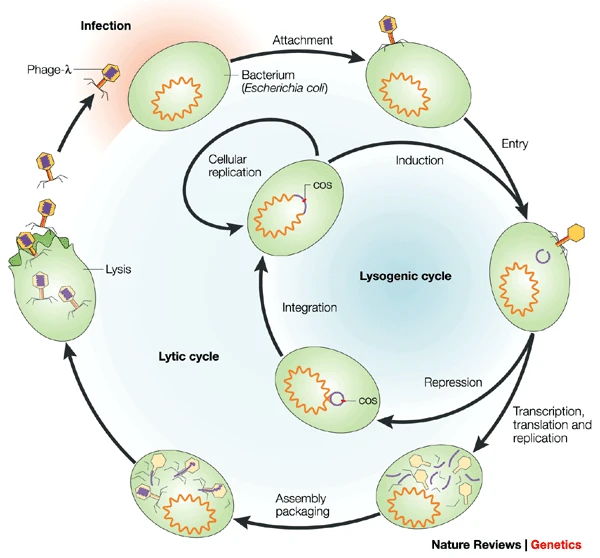
\includegraphics[width=0.5\linewidth]{Figures/phage_life_cycle.png}
    \caption{Life cycle of a phage, inside and outside a bacteria cell. Significant steps in the life cycle of a phage include the infection stage, integration, replication, and lysing process. Figure sourced from \citet{campbellFutureBacteriophageBiology2003}. }
    \label{fig:phage_life_cycle}
\end{figure}

\subsection{Phage's Role in the Environment}
Phages play a large role in the ecosystem. 
As bacteria die, for example through lysis, they release resources into the environment for other bacteria and plants to use. 
This turns over resources like nitrogen and carbon for other sources to use. 
Phages also help mediate horizontal gene transfer, disperse pathogenic diseases, and spread antibiotic resistance \cite{al-shayebCladesHugePhages2020}. 
Phages directly alter bacteria population diversity and population fitness by introducing new ways for bacteria to mutate \cite{brownEcologicalFunctionalRoles2022}. 
There are about $10^6$ bacteria cells/ml and $10^7$ phages/ml of marine water. 
About 5\% of any bacteria are currently infected and about 15\% of daily bacterial death can be attributed to phages \cite{chibani-chennoufiPhageHostInteractionEcological2004}. 


Phage populations grow by infecting their hosts, but they can also degrade, e.g., by UV. 
UV is a large factor of deactivating marine phages, causing up to a 5\% reduction in phage infectivity per hour \cite{chibani-chennoufiPhageHostInteractionEcological2004}. 

\subsubsection{Phages and Controlling Bacterial Blooms}
Phages could potentially be used to control \textit{Cyanobacteria} (blue-green algae) blooms in the environment \cite{colomaFrequencyVirusresistantHosts2019}. 
\textit{Cyanobacteria} cause damage to aquatic life by consuming resources and oxygen, starving aquatic life and negatively affect human health. 
There is hope that phages can be used to biologically control water quality in waste water treatment plants and in the environment without the use of harsh chemical processes what would otherwise pose environmental and health hazards \cite{krysiak-baltynSimulationPhageDynamics2017, tuckerIdentificationCyanophageMaLBP2005}. 
More information about controlling \textit{Cyanobacteria} can be read in \Cref{sec:AppendixB:environmental_protection}. 

\section{Phage Cocktails and Human Health}
There is particular interest in phage applications in human and animal health, called phage therapy. 
There are about 100 trillion microbes across 5,000 different types of bacteria strains in the human gut. 
The phages will target the specific bacteria of interest, for example \textit{E. Coli}, but it will not affect the other bacteria found in the gut of the human body. 
Antibiotics indiscriminately affect any bacteria disrupt the intricate ecosystem of the gut microbiome, acting as a scorched-earth mechanism. 
Antibiotics have also faced the challenge that bacteria are growing resistance to it, making the antibiotic less effective in the future \cite{odonkorBacteriaResistanceAntibiotics2011, volkovaEffectsEarlylifePenicillin2021}. 
Phages on the other hand specifically target a specific bacterial strain. 
Antibiotic resistant bacteria are typically less resistant to phages. 
The bacteria cell typically has a trade-off between antibiotic resistance and phage resistance. 
So by designing phages to be highly infective, there is hope that the phage-resistant bacteria will lose the antibiotic resistance to counter the phages \cite{laurePhageResistancemediatedTradeoffs2022, zhaoPhagedrivenCoevolutionReveals2024}. 
\Cref{sec:AppendixB:phage_therapy_and_antibiotics} goes more in depth on how phages can be used in a healthcare setting. 

\section{Potential Applications of Phages}
Phages have many uses in an industrial setting. 
Similarly, phage therapies can be used as a preventative method, by preventing the spread of common bacteria in livestock by dosing the animal feed with the phage pills. 
Farmers often raise livestock in tight spaces with a lack of sanitation facilities, increasing the risk of a disease spreading. 
 
Phages can be used to control the growth of bacteria like \textit{Salmonella} while producing food in a factory \cite{sofferBacteriophagesSafelyReduce2016, kowalskaFreshVegetablesFruit2023}. 
\Cref{sec:AppendixB:controlling_foodborne_bacteria} in \Cref{AppendixB} goes into more detail about using phages to control foodborne bacteria. 

\section{Modelling Phages in a Complex Community}
What we know about phages mechanistically often comes from well researched bacteria in a lab like \textit{E. coli} and its phages, and what we know about phages in the environment comes from metagenomic surveys. 
Making the connection between the mechanistically and metagenomic models, which would allow us to make and test different models, is the difficult part. 
Because of this, we need mathematical models to help bridge the gap between the lab and the environment. 

There have been previous attempts to model the complex dynamics of the populations between phages, bacteria, and resources, with the environment using Ordinary Differential Equations (ODE) and Delay Differential Equations (DDE).
Not every interaction in the complex community can be identified, and if an interaction has been identified, the associated parameter values need to be experimentally derived. 

There are two main ways to model phage-bacteria dynamics: spatially and non-spatially.
In a spatial model phages and bacteria can move through space and interact with their neighbors. 
Partial differential equations (PDE) and cellular agent-based models (ABM) have been used to model spatial interactions.
Spatial models lead to more computationally complex models, but can result in more biologically realistic results. 

By contrast, ODE and DDE models describe non-spatial models. 
In a non-spatial model, the bacteria and phages are assumed to be in a well-mixed solution and no distinctions are made in regard to neighbors or distances to other entities. 
Interactions are simplified to a probabilistic approach, where a percentage $p$ of entities interact with one another at time step $t$.
Non non-spatial models are easier to develop, understand, and are more effective in modeling large populations, at the cost of losing spatial information. 

For this thesis, the focus will be modelling resource, phage, and bacteria interactions using an ODE model. 
A phage-bacteria-resource system is described as an $p\times b \times r$ system, meaning $p$ phages, $b$ bacteria, and $r$ resources. 
Current modelling methods have mainly stayed with $1\times 1 \times 1$ models, meaning 1 phage, 1 bacteria, and 1 resource. 
This thesis aims to develop a simulation framework that can model any $p\times b \times r$ ODE system. 

\section{Software Overview}
The project is divided into three logical parts, with an optional fourth part.
The first section is to create the network interaction. 
Here the user of the software can define the number of resources, phages, and bacteria, who interacts with who, and the strength and type of interactions. See \Cref{sec:network_creation_tool} for further information. 
In \Cref{sec:simulation_framework}, the user uploads the network model and parameters and as output receives the time data and population data as an array. 
\Cref{sec:visualization_framework} allows the user to interact with \Cref{sec:network_creation_tool} and \Cref{sec:simulation_framework} with a dashboard. 
The user can graphically edit the attribute values of the edges and nodes of the network, and the user can run more advanced visualizations, for example by changing a parameter value and seeing how that affects the population count. 
There are a few plots included out of the box that the user can test. 
The plots offered in part 3 offer interactivity like hiding and showing lines and dots, zooming in and out, and hovering over the lines and dots to show more details of the data. 

Finally, the user can optionally run multiple simulations and download the data to their disk to create their own custom visualizations using \Cref{sec:custom_visualizations_and_framework}. 
The visualizations created in \Cref{sec:visualization_framework} can theoretically be recreated in \Cref{sec:custom_visualizations_and_framework}. 
The user can choose the same parameter values used for a specific plot in \Cref{sec:visualization_framework}, run the simulation (under the \Cref{sec:ultimate_analysis} section), download the data, and reimplement the graphs. 

The user can use the tool themselves by importing the Python classes in their own code and initializing the classes and passing the appropriate data. 